\documentclass[aspectratio=169]{beamer}
\usepackage{graphics,amssymb,amsfonts,amsmath}
\usepackage{tikz}
\DeclareGraphicsExtensions{.jpg,.pdf,.mps,.png}
\usepackage[latin1]{inputenc}
\usepackage[brazil]{babel}
\usepackage[normalem]{ulem}
\usepackage{pgfpages,enumerate,hyperref}
\usepackage{palatino}   %Fonte sem serifa.
\usepackage{ragged2e}   %Par\'agrafo justificado.
\usepackage{minted}
\usetheme{CambridgeUS}
\usecolortheme{lily}
\usefonttheme[onlymath]{serif}

%colocando número de p\'aginas no slide.
\setbeamertemplate{footline}[frame number]

% desativando os botoes de navegacao.
\beamertemplatenavigationsymbolsempty

%Tela cheia
%\hypersetup{pdfpagemode=FullScreen}

% Layout da p\'agina
\hypersetup{pdfpagelayout=SinglePage,urlcolor=blue,colorlinks=true}

\title[\sc{Django}]{Django + Python}
\author{R\'egis da Silva\\ e\\ Jos\'e Aciole}
\institute{SENAC}
\date{\today}

\begin{document}
\justifying %Par\'agrafo justificado.

%Neste caso insere somente no primeiro slide.
{%
%\usebackgroundtemplate{\centering \vspace*{5cm} 
\includegraphics[width=\paperwidth]{figuras/djangoPython}}

\usebackgroundtemplate{%
\vbox to \paperheight{\vfil\hbox to \paperwidth{\hfil
\includegraphics[width=\paperwidth]{figuras/djangoPython}\hfil}\vfil}
}

  \begin{frame}
	\titlepage
  \end{frame}
}

\section{Django}

\subsection{Python}

\begin{frame}\frametitle{Introdu\c c\~ao}
	\begin{itemize}
		\item Python - linguagem de programa\c c\~ao de alto n\'ivel, interpretada, orientada a objetos e de tipagem din\^amica e forte.
		\item Django - framework de desenvolvido web.
	\end{itemize}
\end{frame}

\begin{frame}[fragile]\frametitle{Um pouco de Python}
	\begin{minted}[bgcolor=green!10]{python}
		lista = [1,-4,5,-3,-8,12]
 		def listaValores():
    		soma = 0
    		for i in lista:
        		if i > 0:
            		soma += i
        		else:
            		print i, 'eh negativo.'
    		print 'Total', soma
		 
		listaValores()
	\end{minted}
\end{frame}

% \begin{frame}[fragile]\frametitle{Um pouco de Python}
% 	\begin{minted}[bgcolor=green!10]{python}
% 		class Pessoa:
%     		nome = 'Leticia'
%     		idade = 28
%     		nota = 8.7
		 
%     		def __init__(self, nome, idade, nota=None):
%         		self.nome = nome
%         		self.idade = idade
%         		self.nota = nota or self.nota
		 
%     		def andar(self, passos=10):
%         		if self.idade > 120:
%             		print 'Nao foi possivel'
%         		else:
%             		print 'Andou \%d passos!'\%passos
		 
% 		a = Pessoa('Regis',34,10)
% 		b = Pessoa('Jose',21,10)
% 		print a.nome, a.idade, a.nota, a.andar(10)
% 		print b.nome, b.idade, b.nota, b.andar(9)
% 	\end{minted}
% \end{frame}

\begin{frame}\frametitle{O que \'e Django}
	O \emph{Django} \'e um framework web desenvolvido em Python.
	
	Foi criado por \emph{Adrian Holovaty} numa ag\^encia publicit\'aria.

	O nome Django foi inspirado no m\'usico de Jazz \emph{Django Reinhardt}.
\end{frame}

\begin{frame}\frametitle{O que \'e Django}
\begin{itemize}
	\item adota o padr\~ao MVC
	\item \^enfase em reusabilidade e plugabilidade
	\item desenvolvimento \'agil
	\item baseado no conceito DRY (\emph{Don't Repeat Yourself}) ``n\~ao se repita''
	\item mapeamento objeto-relacional ORM
	\item orienta\c c\~ao \`a objeto: classes, atributos, m\'etodos, heran\c ca, ...
	\item sistema de administra\c c\~ao
	\item sistema de templates
	\item c\'odigo aberto (\emph{open source})
\end{itemize}
\end{frame}

\begin{frame}\frametitle{MVC x MTV}
	\begin{figure}[h]
	  \centering
  		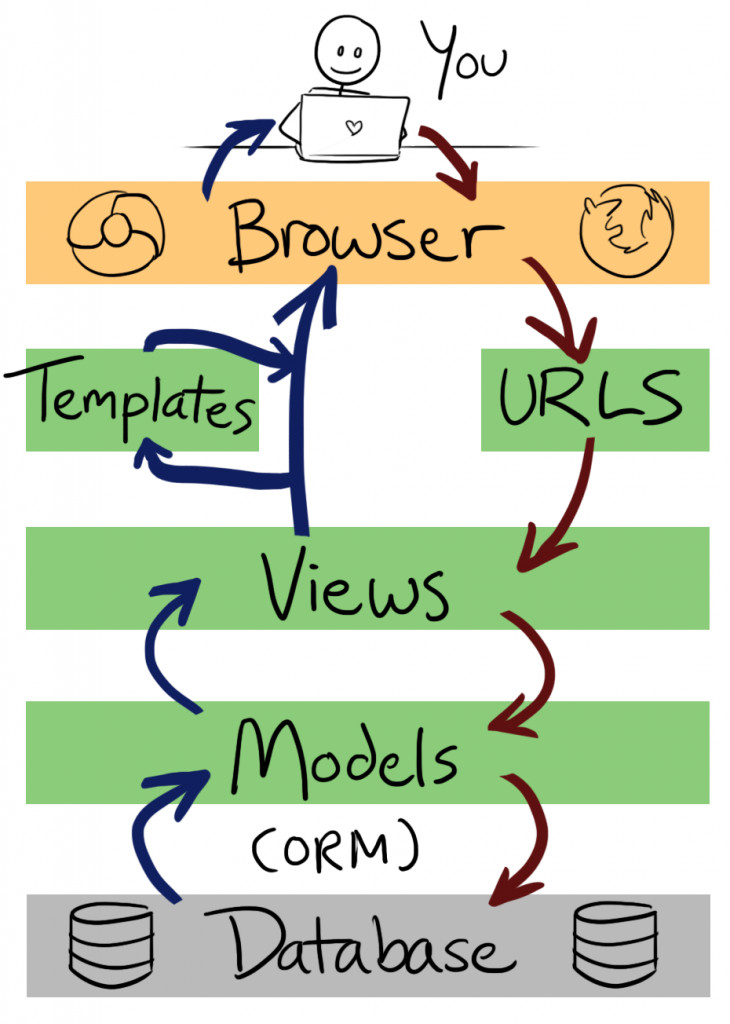
\includegraphics[height=.8\paperheight]{figuras/mtv-diagram}
	\end{figure}
\end{frame}

\begin{frame}\frametitle{MVC x MTV}
	\begin{figure}[h]
	  \centering
  		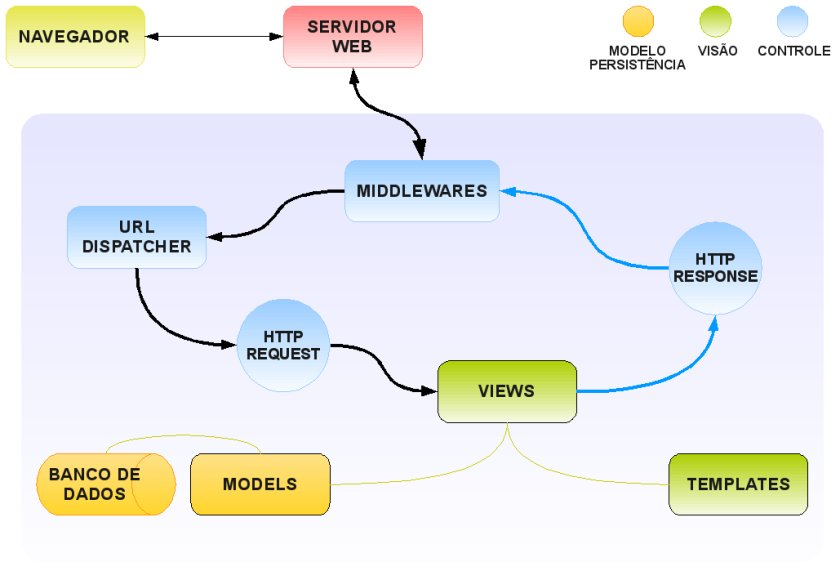
\includegraphics[height=.8\paperheight]{figuras/fluxo-no-mvc}
	\end{figure}
\end{frame}

\begin{frame}\frametitle{Models}
\begin{itemize}
	\item camada de abstra\c c\~ao do banco de dados
	\item definem as entidades do sistema
	\item cada atributo de classe do modelo representa uma coluna do banco de dados
	\item \'e onde acontece o ORM
\end{itemize}
\end{frame}

\begin{frame}\frametitle{Criando um modelo}
	\begin{figure}[h]
	  \centering
  		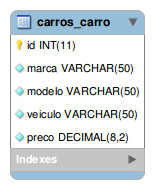
\includegraphics[height=.4\paperheight]{figuras/relacionamentoCarro}
	\end{figure}
\end{frame}

\begin{frame}[fragile]\frametitle{Criando um modelo}
	\inputminted[bgcolor=green!10]{python}{carros_projeto/carros/models.py}
\end{frame}

\begin{frame}[fragile]\frametitle{settings.py}
	\begin{minted}[bgcolor=green!10]{python}
		DATABASES = {
    'default': {
        'ENGINE': 'django.db.backends.mysql', # Add 'postgresql_psycopg2', 'mysql', 'sqlite3' or 'oracle'.
        'NAME': 'carros',                      # Or path to database file if using sqlite3.
        # The following settings are not used with sqlite3:
        'USER': 'root',
        'PASSWORD': '123456',
        'HOST': 'localhost',                      # Empty for localhost through domain sockets or '127.0.0.1' for localhost through TCP.
        'PORT': '',                      # Set to empty string for default.
    }
}
	\end{minted}
\end{frame}

\begin{frame}\frametitle{URL dispatcher}
\begin{itemize}
	\item utiliza URLs limpas e elegantes
	\item Django permite que voc\^e defina as URLs da maneira que quiser
\end{itemize}	
\end{frame}

\begin{frame}[fragile]\frametitle{urls.py}
	\begin{minted}[bgcolor=green!10]{python}
from django.conf.urls import patterns, include, url

# Uncomment the next two lines to enable the admin:
from django.contrib import admin
admin.autodiscover()

urlpatterns = patterns('',
    url(r'^admin/', include(admin.site.urls)),
    url(r'^$', 'carros.views.index', name='home'),
)

	\end{minted}
\end{frame}

\begin{frame}\frametitle{Views}
	Uma \emph{view} \'e simplesmente uma fun\c c\~ao \emph{python} que recebe uma \emph{requisi\c c\~ao} e retorna uma \emph{resposta} web.

	Equivale ao \emph{controller} de outros frameworks.
\end{frame}

\begin{frame}[fragile]\frametitle{views.py}
	\begin{minted}[bgcolor=green!10]{python}
		from django.shortcuts import render_to_response
		from carros.models import Carro

		def index(request):
			return render_to_response('carros/index.html',{
				'carros': Carro.objects.all().order_by('id')
		})
	\end{minted}
\end{frame}

\begin{frame}\frametitle{Templates}
\begin{itemize}
	\item O uso de \emph{template} no \emph{Django} proporciona facilidade e flexibilidade
	\item um \emph{template} cont\'em vari\'aveis e \emph{tags}, quando o \emph{template} \'e avaliado essas vari\'aveis s\~ao substitu\'idas por valores
	\item Equivale ao \emph{view} de outros frameworks.
\end{itemize}	
\end{frame}

\begin{frame}[fragile]\frametitle{Vari\'aveis}
Acessando o valor de uma vari\'avel

\begin{minted}[bgcolor=green!10]{python}
{{ variavel }}
\end{minted}

Acessando atributos

\begin{minted}[bgcolor=green!10]{python}
{{ carro.marca }}
\end{minted}

Tags

\begin{minted}[bgcolor=green!10]{python}

\end{minted}

\begin{itemize}
 	\item tags podem criar texto na sa\'ida
 	\item podem aplicar \emph{loops} ou l\'ogica
\end{itemize}

\end{frame}

\begin{frame}[fragile]\frametitle{Sintaxe mais completa}
\begin{minted}[bgcolor=green!10]{python}

	...

\end{minted}

Coment\'arios

\begin{minted}[bgcolor=green!10]{python}
{# comentario #}
\end{minted}
\end{frame}

%Falar sobre QuerySet

\begin{frame}[fragile]\frametitle{Exibindo dados}
	\begin{minted}[bgcolor=green!10]{html}

	<table>
		<tr>
			<td>{{current.marca}}</td>
			<td>{{current.modelo}}</td>
			<td>{{current.veiculo}}</td>
			<td>{{current.preco}}</td>
		</tr>
	</table>

	\end{minted}
\end{frame}

\begin{frame}\frametitle{Exibindo dados}
	\begin{figure}[h]
	  \centering
  		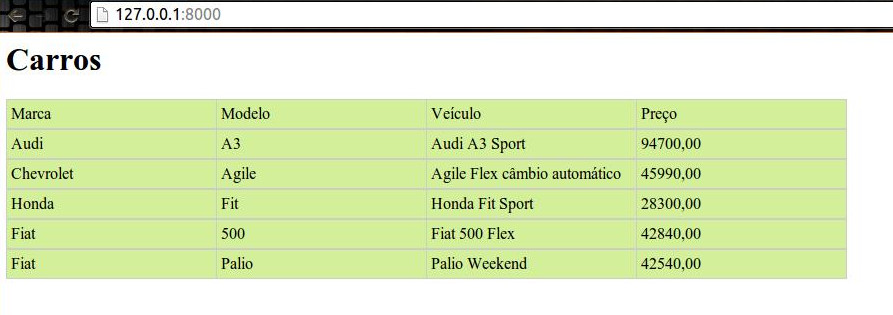
\includegraphics[height=.5\paperheight]{figuras/pagina}
	\end{figure}
\end{frame}

\begin{frame}\frametitle{Forms}
\begin{itemize}
	\item o \emph{forms} \'e uma biblioteca do \emph{django} para cria\c c\~ao de formul\'arios
	\item \'e poss\'ivel gerar um formul\'ario automaticamente atrav\'es de um \emph{model}
	\item possui regras de valida\c c\~ao autom\'atica para cada tipo de campo
\end{itemize}
\end{frame}

\begin{frame}\frametitle{Programas e bibliotecas auxiliares}
\begin{itemize}
	\item virtualenv - para isolar os ambientes de cada projeto
	\item pip - para instala\c c\~ao de pacotes
	\item south - para migra\c c\~oes de modelos de dados
	\item git - versionamento
	\item fabric - deploy
\end{itemize}
\end{frame}

\begin{frame}\frametitle{Programas usados}
	\begin{center}
      \begin{tabular}{r|l}
		SO & Linux (Ubuntu 13.10) \\
		Linguagem & Python \\
		Framework & Django \\
		SGBD & MySQL \\
		Front-End do SGBD & Workbench \\
		Editor & Sublime Text 3 \\
		Compilador & Shell do sistema (terminal) \\
		Versionamento & Git \\
		Apresenta\c c\~ao & LaTeX \\
      \end{tabular}
    \end{center}
\end{frame}


\begin{frame}\frametitle{Sites feitos com Django}
	\url{http://www.djangosites.org/tag/djangobrasil/}
	
	\url{http://blog.glaucocustodio.com/2013/01/10/comecando-com-django-instalando-e-rodando-no-linux/}
	
	\url{http://blog.glaucocustodio.com/2012/08/09/desenvolvimento-em-camadas-com-mvc/}
	
	\url{http://www.djangobrasil.org/}
	
	\url{https://www.djangoproject.com/}
	
	\url{http://osantana.me/2008/03/03/ambiente-isolado-para-python-com-virtualenv/}
	
	\url{http://www.djangosites.org/}
	
	\url{http://imasters.com.br/artigo/10824/desenvolvimento/aplicacoes\_rapidas\_para\_web\_com\_django/}
\end{frame}

\begin{frame}\frametitle{Obrigado}
	\centering
	\url{https://github.com/rg3915/django}
\end{frame}

\end{document}